\documentclass[12pt]{article}

\usepackage{amsmath, mathtools}
\usepackage{amsfonts}
\usepackage{amssymb}
\usepackage{graphicx}
\usepackage{colortbl}
\usepackage{xr}
\usepackage{hyperref}
\usepackage{longtable}
\usepackage{xfrac}
\usepackage{tabularx}
\usepackage{float}
\usepackage{booktabs}
\usepackage{caption}
\usepackage{pdflscape}
\usepackage{afterpage}

\usepackage[round]{natbib}

\hypersetup{
    bookmarks=true,         % show bookmarks bar?
    colorlinks=true,       % false: boxed links; true: colored links
    linkcolor=red,          % color of internal links (change box color with linkbordercolor)
    citecolor=green,        % color of links to bibliography
    filecolor=magenta,      % color of file links
    urlcolor=cyan           % color of external links
}

%% Comments

\usepackage{color}

\newif\ifcomments\commentstrue %displays comments
%\newif\ifcomments\commentsfalse %so that comments do not display

\ifcomments
\newcommand{\authornote}[3]{\textcolor{#1}{[#3 ---#2]}}
\newcommand{\todo}[1]{\textcolor{red}{[TODO: #1]}}
\else
\newcommand{\authornote}[3]{}
\newcommand{\todo}[1]{}
\fi

\newcommand{\wss}[1]{\authornote{blue}{SS}{#1}} 
\newcommand{\plt}[1]{\authornote{magenta}{TPLT}{#1}} %For explanation of the template
\newcommand{\an}[1]{\authornote{cyan}{Author}{#1}}

%% Common Parts

\newcommand{\progname}{Mechtronics Enigeering} % PUT YOUR PROGRAM NAME HERE
\newcommand{\authname}{Team 32, Wingman
\\ Edward He
\\ Erping Zhang
\\ Guangwei Tang
\\ Peng Cui
\\ Peihua Jin } % AUTHOR NAMES                  

\usepackage{hyperref}
    \hypersetup{colorlinks=true, linkcolor=blue, citecolor=blue, filecolor=blue,
                urlcolor=blue, unicode=false}
    \urlstyle{same}
                                


\title{Software Requirements Specification\\\progname}

\author{\authname}

\date{}

\begin{document}

\maketitle

\newpage
\begin{table}[hp]
\caption{Revision History} \label{TblRevisionHistory}
\begin{tabularx}{\textwidth}{llX}
\toprule
\textbf{Date} & \textbf{Developer(s)} & \textbf{Change}\\
\midrule
2022-10-05 & Edward He, Erping Zhang & Revision 0\\
& Guangwei Tang, Peng Cui & \\
& Peihua Jin & \\\\
2022-11-20 & Guangwei Tang, Erping Zhang & Update functional and non-functional Requirements\\\\
2023-1-16 & Peng Cui, Edward He & Change FSM and update context diagram\\\\
2023-3-26 & Peihua Jin & Change some incorrect Concepts\\\\
2023-4-3 & Peihua Jin, Peng Cui & Update control and monitored variables, check for grammar errors\\
\bottomrule
\end{tabularx}
\end{table}


This document is a modified Volere template and has been adopted according to project needs. Since this is a Mechatronics project, some subsections are different comparing to the original Volere template. The document follows the general organization of the Volere template with some additional sections to better suit for Mechatronics. 

Neglected subsections: the hands-on users of the product, persona, priorities assigned to users, users participation, maintenance users and service technicians,implementation environment of the current system, partner or collaborative applications, off-the-shelf software, anticipated workplace environment, enterprise constrains, relevant facts, business rule.
\newpage


\tableofcontents

\newpage



\listoftables
\listoffigures

\newpage

\pagenumbering{arabic}



\begin{table}

\end{table}

\section{Project Drivers}

\subsection{The Purpose of the Project}
The purpose of the project is to build a Mechatronics system called "SmartVault" that is able to assist user in finding their belongings in a given area. 
\subsection{The Purpose of the Document}
This document is intended to provide detailed set of requirements project SmartVault. The documentation will cover the functionality of the system and the requirements that the system is expected to fulfill. In addition to the function requirements of software system, non-functional requirements will also be included in this document. Any additional useful information for building the system is also covered and written in details. This document is used as a reference and guideline for the development of the system and is to ensure that the built system is fulfilling the necessary requirements and meeting the desired goals.
\subsection{The Stakeholders}

\subsubsection{The Client}
\begin{itemize}
    \item Dr. Spencer Smith, professor from McMaster University, Computing and Software department. 
\end{itemize}

\subsubsection{The Customers}
\begin{itemize}
    \item people who often can't find their belongings due to poor organization
   	\item people who has bad memory  
\end{itemize}
\subsubsection{Other Stakeholders}
N/A
\section{Project Constraints}
\subsection{Mandated Constraints}
\begin{center}
    \begin{tabular}{|| p{3cm} || p{8cm} ||}
    \hline
    MC1 & The cost of purchasing components and parts should not exceed \$750  \\
    \hline
    Description & Cost are restricted as a hard requirement in project designing stage \\
    \hline\hline
    MC2  & The submission date of the complete project design is by the end of academic year\\
    \hline
    Description & Based on course requirement, project has a solid deadline\\
    \hline\hline
    MC3 & The design should be an integration of hardware and software\\
    \hline
    Description & As part of the project hard requirement for Mechatronics group, the design can not be all software based \\
    \hline\hline
    \end{tabular}
\end{center}
\subsection{Naming Conventions and Terminology}
	\subsubsection{Definitions of All Terms}
		\begin{center}
    		\begin{tabular}{|| p{3cm} || p{8cm} ||}
   			 	\hline
    			Object& The physical objects need to be tracked and searched in the room  \\
   				\hline
    			Camera Mount & The motorized mount that hold the camera and adjust the angle of the camera view \\
    			\hline
   				 Servo  & An electromagnetic device that converts electricity into precise controlled motion by use of negative feedback mechanisms\\
    			\hline
   			 Field Oriented Control(FOC) & A variable-frequency drive control method in which the stator currents of a three-phase AC or brushless DC electric motor are identified as two orthogonal components that can be visualized with a vector\\
    			\hline
    			Relocation & The change of the position or location of an object in the room\\
    			\hline
   				Controller Board & A hardware chip set with General Purpose Input and Output ports, which send data from camera to laptop and control the rotation of camera mount\\
   				\hline
   				Serial Communication & A communication method that uses one or two transmission lines to send and receive data, and that data is continuously sent and received one bit at a time\\
   				\hline
   				User Interface & A embedded software program that allow user to interact with the searching system\\
   				\hline
   				Camera & The device that collect video data and send the data to rest of the system\\
   				\hline 
   				Human Detection & The action that system can recognize the existance of human shown in the room\\
   				\hline
   				File Storage & The physical space in system which record information about each object\\
    \hline\hline
    \end{tabular}
\end{center}
	



\subsection{Relevant Facts and Assumptions}




\subsubsection{User Characteristics}
The users of SmartVault are people who have trouble finding their belongings in their daily lives. It is preferred that the user to have general knowledge of what is presented in the designated area. Users should be familiar and comfortable with technology. At minimum, the users should be able to read, type and navigate on a web-page. 
\subsubsection{Reader Characteristics}
The intended readers for this document are the developers responsible for developing SmartVault. Dr.Smith, a professor at McMaster University and his teaching team will also be the intended reader of this document. The document is written in a technical manner and requires the reader to possess both software and hardware knowledge. The reader should be familiar with image processing and the ability to understand the basic logic of object detection. The reader should also understand the software design cycle and the steps taken to develop a complete software program. In order to fully understand the document, it is suggested that the reader has the ability to read and comprehend the communication and control system between a software program and hardware device. 
\subsubsection{Assumptions and Dependencies}
\textbf{AD1:} The user can perform simple computer operations.\\
\textbf{Rationale:} The user can type, moving mouse and clicking on the window.\\\\
\textbf{AD2:} The user can understand English.\\\\
\textbf{AD3:} The operation of the project should take place indoors with adequate lighting.\\\\
\textbf{AD4:} All objects can be seen by the product without hiding.\\\\
\textbf{AD5:} The general motion of the user can be seen by the device. 
\section{Functional Requirements}


\subsection{The Scope of the Work}
The following picture shows the design of the context diagram of the project. In this diagram, the user can interact with the SmartVault by logging in successfully. The user can also provide timing information about the object to get feedback from SmartVault. A camera will be mounted inside the room and it will keep sending images to Smatvault for image processing. The motor is used to changes the angular position of the camera so that the desired location is achieved. After SmartVault has done image processing, it will update the data in the file storage and will extract information when the user needs it. 
\subsubsection{The Context of the Work}
\begin{figure}[H]
    \centering
    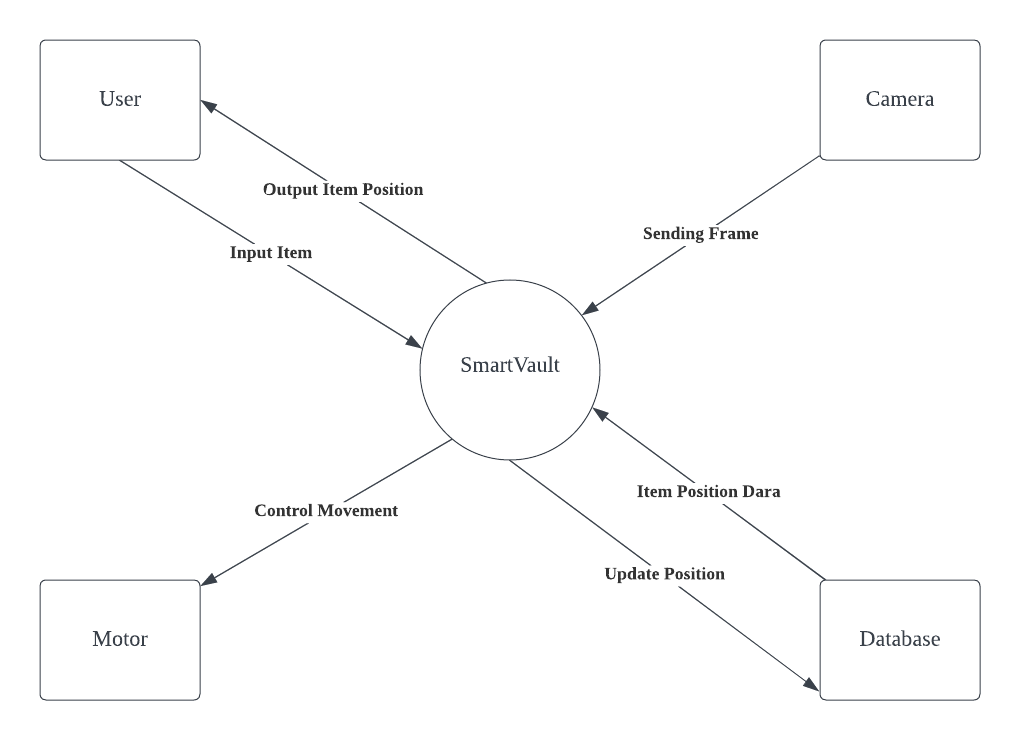
\includegraphics[scale=0.7]{Context.png}
    \caption{Context of Work}
\end{figure}
\subsubsection{Work Partitioning}
The following table shows the work partitioning of the project. all possible types of those events are included in the table. A functional Decomposition Diagram is also shown to show the whole working condition of the project. 
\begin{table}[H]
\caption{Event List} 
\begin{tabularx}{\textwidth}{XXX}
\toprule
\textbf{Event Name} & \textbf{Input and Output} & \textbf{Types of Input or Output}\\
\midrule
User input & Item description(in) & Username and password, timing information about the object want to find, operational  actions\\\\
UI output &  Information(out) & Item pictures, picture showing the position of the selected item.\\\\
Provide item position & Item position (out) & Item pictures, picture about the position of the object\\\\
Live feed from camera & Live frames(in) & pictures taken by the camera.\\\\
Motor Control& Degree and direction of rotation (out) & rotating angle and speed.\\\\
Update file & New item position(out) & Replace or add position data for an item in the database.\\\\
Acquire position & Item timing information & time interval information related to the item.\\\\

\bottomrule
\end{tabularx}
\end{table}

\begin{figure}[H]
    \centering
    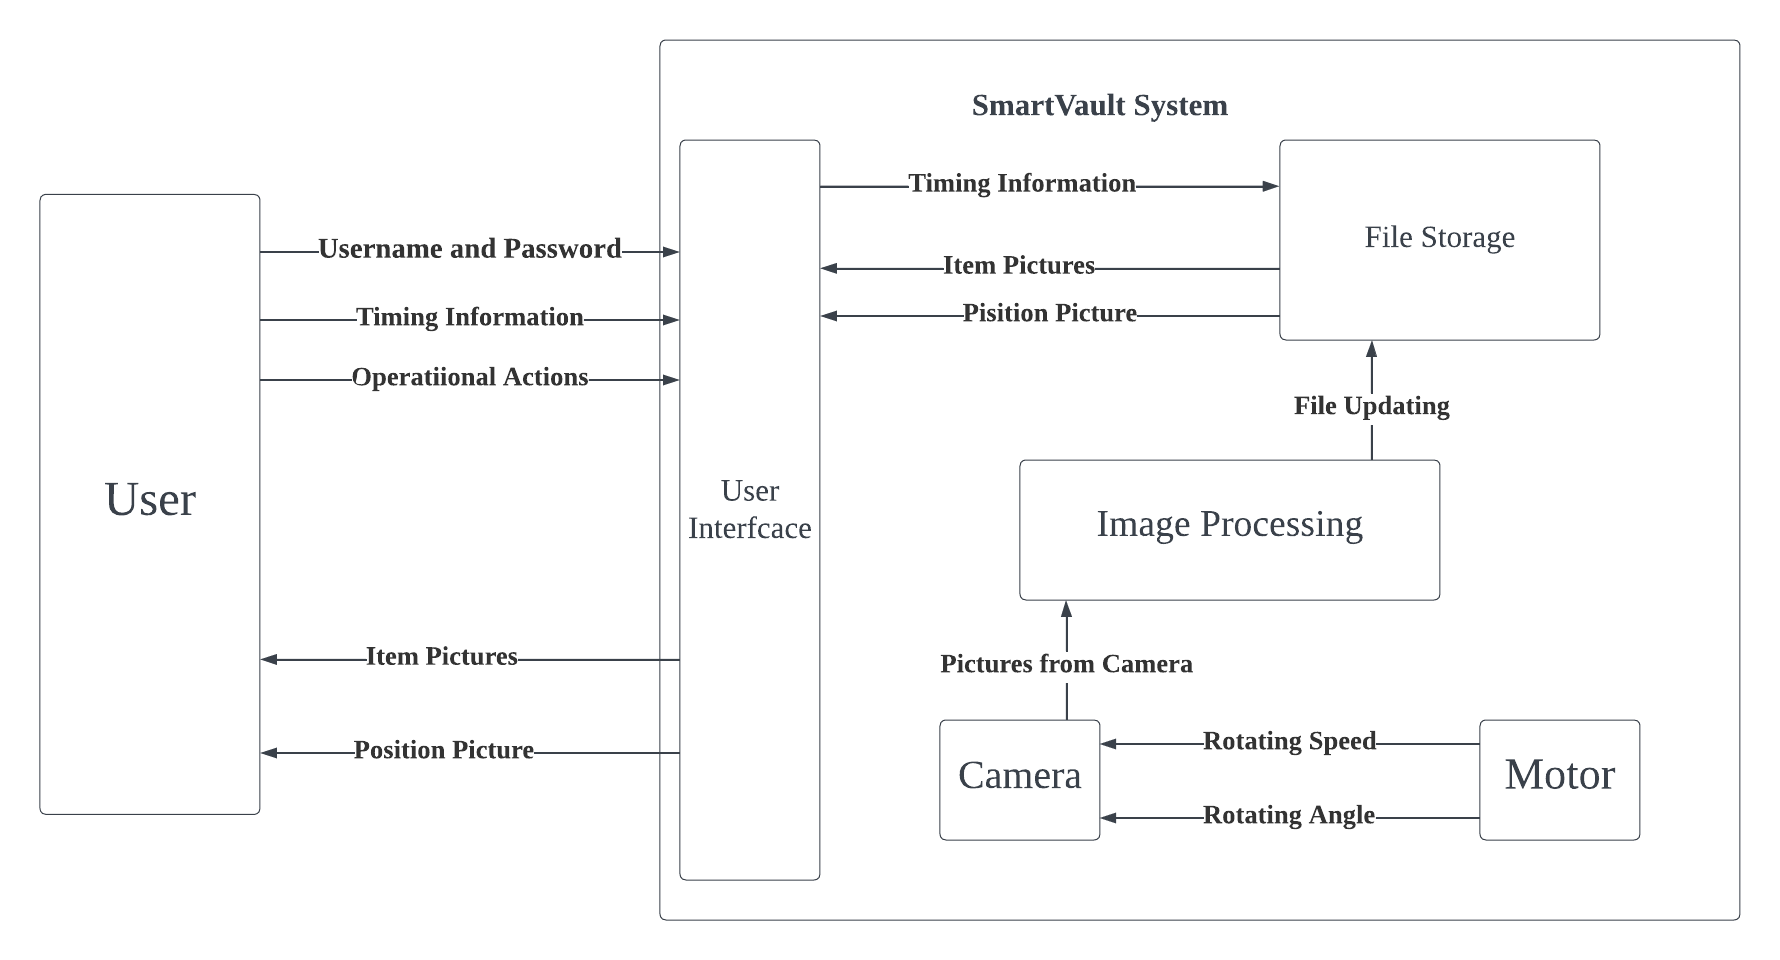
\includegraphics[scale=0.3]{Function_Decom.png}
    \caption{Functional Decomposition Diagram}
\end{figure}

\subsection{The Scope of Product}
\subsubsection{Finite State Machine Description}
To make the behaviour of the product to achieve the target task, the Finite State Machine is created to describe the behaviour with detailed description provided after the picture. 
\begin{figure}[H]
    \centering
    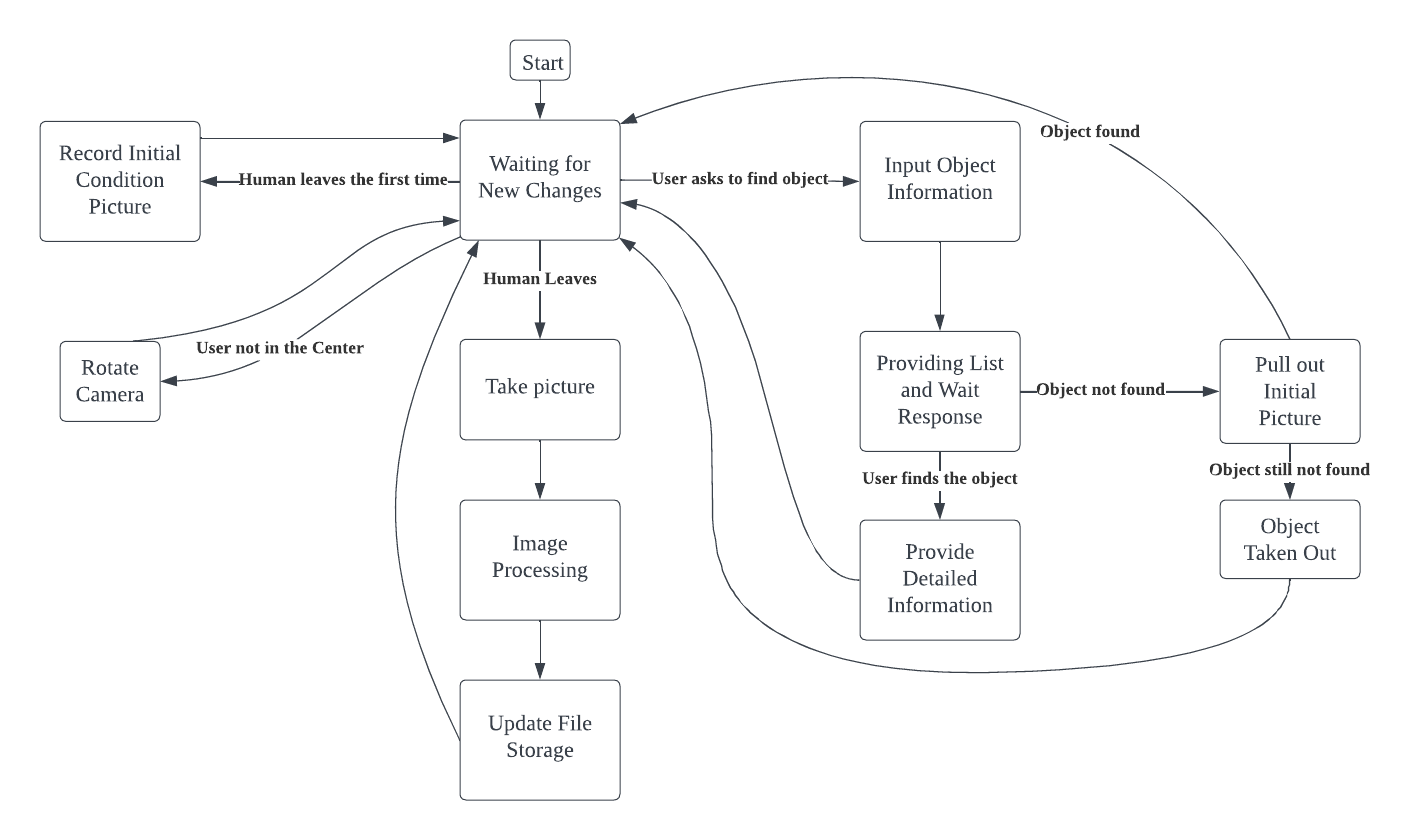
\includegraphics[scale=0.6]{FSM.png}
    \caption{The Picture of Finite  State Machine}
\end{figure}
\noindent\textbf{Record Initial Condition:} When the user leaves the room for the first time, the device will take a picture of the room as the initial position information for each object and save it to the file storage module. \\\\
\textbf{Waiting for New Changes:} The device will wait for future changes to the system. \\\\
\textbf{Take Picture:} If the user leave the room after taking the initial picture, the camera will take another picture and send both pictures to the image processing module.  \\\\
\textbf{Image Processing:} The system will take the difference of the two pictures, identify new existence or position change of the objects shown in the image.\\\\
\textbf{Update File Storage:} The device will record the updated information (including time, Location, picture of object, and so on) of the object into the file storage module.\\\\
\textbf{Input Object Information} When the user want to find one object in the room, the user interface will ask the user to input information of the object (like size, color, last time saw it, and so on).\\\\
\textbf{Providing List and Wait Response:} After the user has input the information, the system will provide a list of objects with pictures that satisfy the input information.\\\\
\textbf{Provide Detailed Information:} When the user find the target object, the device will display the detailed information about the object like showing the current location on the screen. \\\\
\textbf{Rotate Camera:} If the device found the human body detected is not in the center of the screen or the camera is covered by something else, it will send signals to the motor to rotate the camera until problem solved. 


\subsubsection{Individual Product Use Cases}
\begin{figure}[H]
    \centering
    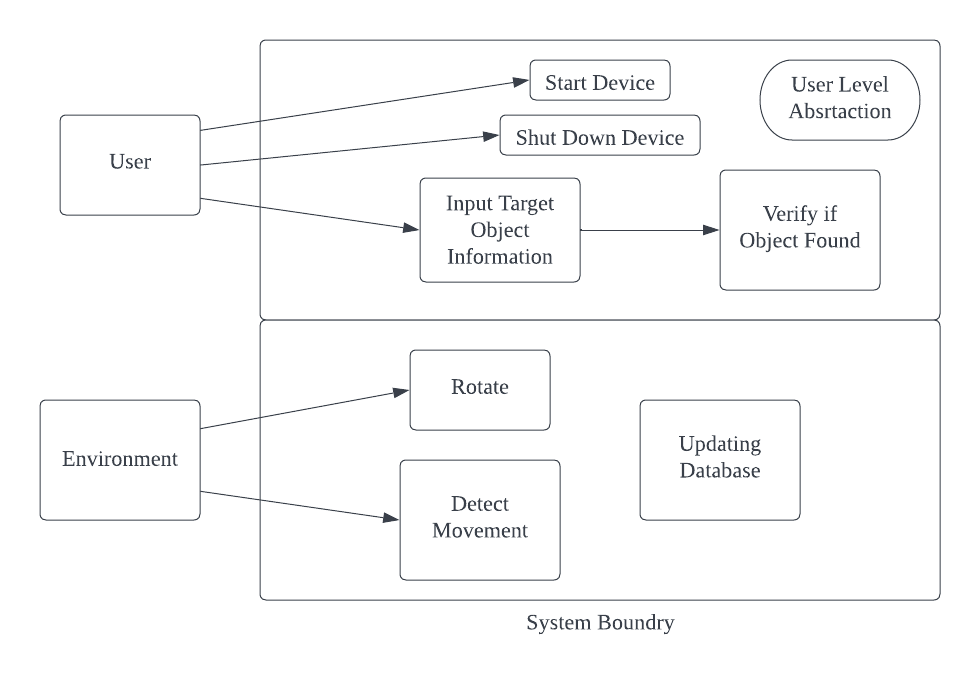
\includegraphics[scale=0.8]{Use.png}
    \caption{The Picture of Use Case Diagram}
\end{figure}
The Use Case Diagram shown above describes some actions that the user can interact with the system. The line in the middle shows the boundaries between user and the internal program. The out-most large box shows the boundary for the whole system. All user can do is just to start and shut down the program. The user can also find the target object by typing the information about the object and verify if the object is found. The system will interact with the environment by rotating its camera and detecting the movement of the object in the room. It will also be able to update its database when the position of the object is changed. 

\subsection{Monitor and Control Variables}
\subsubsection{Monitor Variable}

\begin{table}[H]
\caption{Table of Monitored Variables} 
\begin{tabularx}{\textwidth}{XXXXX}
\toprule
\textbf{Variable Name} & \textbf{Type} & \textbf{Unit} & \textbf{Range} & \textbf{Comment} \\
\midrule
Detected Object position & int & pixel sizes for an image & size of the whole picture & The relative location of the detected object related to the frame image.\\\\
Human position & list of int & pixel sizes of an image & size of the whole picture & a structure shows human body\\\\
Detected Object characteristic & not applicable &  based on software libraries & not applicable & The feature of the detected object\\\\
Detected Object last seen time & time & timing values from seconds to days & 1 day to 365 days & the timing information used to search for an object\\\\
\bottomrule
\end{tabularx}
\end{table}

\subsubsection{Control Variable}

\begin{table}[H]
\caption{Table of Control Variables} 
\begin{tabularx}{\textwidth}{XXXXX}
\toprule
\textbf{Variable Name} & \textbf{Type} & \textbf{Unit} & \textbf{Range} & \textbf{Comment} \\
\midrule
Degree of movement of the motor & float & degrees & 2 degrees to 180 degrees & the angular movement can be made by the motor.\\\\
Direction of movement of the motor & not applicable & not applicable & either positive or negative & the direction that the motor can move\\\\
Speed of turning of the motor &  float & degrees per second & 10 to 90 degrees per second & the speed of the motor\\\\
\bottomrule
\end{tabularx}
\end{table}

\subsection{Functional Requirements}
The following are the functional requirements of the project. They are separated into 2 main parts: Image Processing and Storage, and User Interface Menu.

\subsubsection{Image Processing and Storage Requirements}
\textbf{IPR1:} The system should be able to identify human's body.\\
\textbf{Rationale:} When human enters the camera frame, the system needs to be able to identify it and presents a strcture on the image.\\\\
\textbf{IPR2:} The system should be able to identify the movement or new existence of different objects. \\
\textbf{Rationale:} By applying Image processing, the system is able to identify those changes.\\\\
\textbf{IPR3:} The system should be able to take a photo once the user leave the room.\\\\
\textbf{IPR4:} The system should be able to differentiate one item from another items which are identified by the system through 3 main parameters, item\_shape, item\_color and item\_size.\\\\
\textbf{IPR5:} The system must be able to store all the photos into a file, and indicate the time when it was taken.\\\\
\textbf{IPR6:} The system must be able to update the file storage module.\\\\
\textbf{IPR7:} The system must be able to name each item with a unique ID.\\\\
\textbf{IPR8:} The system should be able to arrange the photos stored in the file in ascending or descending order according to the time it was taken.\\\\
\textbf{IPR9:} The system should be able to arrange the photos stored in the file in ascending or descending order according to their IDs.

\subsubsection{User Interface Menu Functional Requirements}
\textbf{UIR1:} The UI should be able to let user to choose whether to highlight a certain item or not.\\\\
\textbf{UIR2:} The UI should be able to let user to switch the ordering method.\\\\
\textbf{UIR3:} The UI should be able to let the user login by inputting correct usernme and password.\\\\
\textbf{UIR4:} The UI must be able to allow the user to view the system's status at any given point in time.\\\\
\textbf{UIR5:} The UI must be able to provide Technical to the user. \\
\textbf{Rationale:} To ensure that the system will remain operational.






\section{Nonfunctional Requirements}
The next paragraphs will talk about about non-functional requirements in the designing of the SmartVault, which will be discussed in several different parts. 
\subsection{Look and Feel Requirements}
\subsubsection{Appearance Requirements}
\textbf{APR1:} The device should not have exposed internal electronic wiring.\\\\
\textbf{APR2:} The sharp corners should not be exposed to the users and should be covered by some soft materials.
\subsubsection{Style}
Not Applicable.
\subsection{Usability and Humanity Requirements}
\subsubsection{Easy of Use Requirements}
\textbf{EUR1:} The device should be easy to installed in the room.\\\\
\textbf{EUR2:} Fonts, blanks and graphics shown on the screen should be big and visible enough for the user to use without inserting wrong information.
\subsubsection{Personalization and Internationalization Requirements}
Not applicable.
\subsubsection{Learning Requirements}
\textbf{LER1:} The software part of the product should be easy to install.\\\\
\textbf{LER2:} The product should be easy to be set up in its working environment.\\
\textbf{Rationale:} The device can identify objects in the room in a short time after powering up.
\subsubsection{Understandability and Politeness Requirements}
\textbf{UPR1:} The graphics used should be readable and visible to the user.\\
\textbf{Rationale:} Easy for clients to find objects that wish to find in the room.
\subsection{Accessibility Requirements}
\textbf{ACR1:} The display window should be concise enough for user to understand
\subsection{Performance Requirements}
\subsubsection{Speed and Latency Requirements}
\textbf{SLR1:} The response time of the product to show the location of the object should be less than 5 seconds.
\subsubsection{Safety-Critical Requirements}
\textbf{SCR1:} The base of the device should be strong enough without falling from the floor.\\\\
\textbf{SCR2:} The device should not infringe on user's privacy.\\\\
\textbf{SCR3:} The normal rotating speed of the motor should be slow enough without hurting people.\\
\textbf{Rationale:} The average rotating speed should be controlled to about 30 degrees per seconds.
\subsubsection{Precision and Accuracy Requirements}
\textbf{PAR1:} The time based value used in the device should be precise to seconds.\\\\
\textbf{PAR2:} The location value used in the device should be precise to whole number.\\\\
\textbf{PAR3:} Other numerical values used in the device should be rounded to one decimal place.
\subsubsection{Reliability and Availability Requirements}
\textbf{RAR1:} The device should not over-rotate to an unexpected angle.\\
\textbf{Rationale:} The range of the angle is set to be -180 degrees to 180 degrees.\\\\
\textbf{RAR2:} The device should be available to work for the whole time of except for maintenance or updating time.
\subsubsection{Robustness or Fault-Tolerance Requirements}
\textbf{RFR1:} The data stored in the file should not be deleted or changed even after the program shuts down.\\\\
\textbf{RFR2:} The device should be able to notify user for an error occurs in the program.\\
\textbf{Rationale:} The user should be notified if he or she has a wrong input or having inappropriate actions.
\subsubsection{Capacity Requirements}
\textbf{CAR1:} The device should be able to store the any information about the location of each object detected from the camera.
\subsubsection{Scalability or extensibility Requirements}
Not applicable.
\subsubsection{Longevity Requirements}
\textbf{LOR1:} The device should store the information about the objects until it is changed into a different environment.
\subsection{Operational and Environmental Requirements}
\subsubsection{Expected Physical Environment}
\textbf{EPE1:} The device is supposed to work in any indoor space.
\subsubsection{Requirements for Interfacing with Adjacent Systems}
Not applicable.
\subsubsection{Productization Requirements}
Not applicable.
\subsubsection{Release Requirements}
No applicable.
\subsection{Maintainability and Support Requirements}
\subsubsection{Maintenance Requirements}
\textbf{MAR1:} The maintenance for the device should be done by the developers.
\subsubsection{Supportability Requirements}
\textbf{SUR1:} The device is supported by any computers supports both C and python programming languages.
\subsubsection{Adaptability Requirements}
Not Applicable.
\subsection{Security Requirements}
\subsubsection{Access Requirements}
\textbf{AER1:} Any one except for the users is not allowed to access the any file that stores the information about the objects in the room.
\subsubsection{Integrity Requirements}
\textbf{INR1:} Data in the files should not be changed unnecessarily.\\\\
\textbf{INR2:} The files are locked when the device shuts down.
\subsubsection{Privacy Requirements}
\textbf{PRR1:} Other users are not allowed to access any file in the computer.\\\\
\textbf{PRR2:} The camera should only work for a specific user.
\subsubsection{Audit Requirements}
Not applicable.
\subsubsection{Immunity Requirements}
Not applicable.
\subsection{Cultural and Political Requirements}
\subsubsection{Cultural Requirements}
Not applicable.
\subsubsection{Political Requirements}
Not applicable.
\subsection{Legal Requirements}
\subsubsection{Compliance Requirements}
\textbf{CPR1:} The performance of the product should not violate the laws that protect the privacy of thee user.
\subsubsection{Standards Requirements}
Not applicable.


\section{Traceability and Priority}
For both functional and non-functional requirements, the dependency matrix is made and priorities are assigned to each requirement. The Traceability matrix and priority table are shown below. In addition, the likelihood change of the requirements and the future plan of the requirements are also shown below.

\subsection{Traceability Matrix}
\begin{table}[H]
\begin{tabular}{|p{0.45\textwidth}| p{0.45\textwidth}|}

\hline Functional Requirement ID & Nonfunctional Requirement ID\\

\hline IPR2, IPR5, IPR6 & LER2\\

\hline IPR8, IPR9, UIR3 & UPR1, PAR2\\
\hline UIR4 & RFR2\\
\hline IPR6, IPR7, IPR8 & CAR1\\
\hline

\end{tabular}
\caption{Requirement Traceability Matrix}
\end{table}

\subsection{Priority Table}
\begin{table}[H]
\begin{tabular}{|p{0.36\textwidth}|p{0.42\textwidth}|p{0.1\textwidth}|}

\hline Functional Requirement ID&Nonfunctional Requirement ID&Priority\\

\hline IPR1, IPR2, IPR3, IPR3, IPR4, IPR5, IPR6, IPR7, UIR1, UIR3 & LER2, UPR1, SCR2, PAR1, PAR2, PAR3, RFR1, RFR2, CAR1, EPE1, INR1, CPR1 & HIGH\\

\hline IPR8, IPR9, UIR2, UIR4 & APR1, APR2, EUR2, ACR1, SCR3, RAR1, RAR2, SUR1, AER1, INR2, PRR1, PRR2 & MID\\

\hline UIR5 & EUR1, LER1, SCR1, MAR1 & LOW\\

\hline

\end{tabular}
\caption{The Priority Table for each Requirement}
\end{table}

\subsection{Likelihood of Changes}
\begin{table}[H]
\begin{tabular}{|p{0.25\textwidth}|p{0.15\textwidth}|p{0.60\textwidth}|}

\hline Requirement ID&Likelihood&Ways to Change\\

\hline IPR2(func)&Likely&The image processing method may be changed to achieve a more accurate result.\\

\hline IPR9(func)&likely&Since time is the easiest way to track an object, the assistance information may be changed so the ordering method may also be changed.\\

\hline UIR1(func)&likely&The device will remember each object that is moved so this function may be useless.\\

\hline UIR2(func)&likely&The sorting method is determined by the program not the user, so the ording method may not depend on the user. \\

\hline EUR1(nonfunc)&likely&The physical installation of the device may be changed after the model is built.\\

\hline SCR1(nonfunc)&likely&The base may be changed when the installation method of the device changed/\\

\hline CAR1(nonfunc)&very likely&The device may only choose information that make the sorting algorithm easier.\\

\hline

\end{tabular}
\caption{Requirements that are likely to change}
\end{table}

\subsection{Requirement Timeline}
\begin{table}[H]
\begin{tabular}{|p{0.5\textwidth}|p{0.5\textwidth}|}

\hline Requirement ID&Finish Date\\


\hline IPR1, IPR3, IPR6, ACR1, PAR1, PAR2, PAR3, SUR1&2022.10.31\\

\hline RFR1, CAR1, AER1, INR1, PRR1, PRR2&2022.11.15\\

\hline IPR2, IPR4, IPR5, UIR1, UIR3, UIR4, LER2, RFR2&2022.11.28\\

\hline EUR2, SLR1, INR2&2022.12.15\\

\hline IPR7, IPR8, IPR9, UIR2, UPR1, SCR2, SCR3, RAR1&2022.12.30\\

\hline EUR1, LER1, SCR1, RAR2, EPE1, MAR1, CPR1&2023.1.15\\

\hline

\end{tabular}
\caption{The Timeline for each Requirement}
\end{table}


\section{Project Issues}

\subsection{Open Issues}

\begin{itemize}
    \item Limit of 180 rotation degree of servo motor
    \item Accuracy of object detection 
    \item How to distinguish two objects with very limited resources
    \item How to recognize the same object in different angles
    \item How to guarantee the stability of the serial communication
\end{itemize}


\subsection{Off-the-Shelf Solutions}
\begin{itemize}

    \item Huskylens - is a AI camera which can learn new objects and recognize them. It has the machine learning technology enables projects to interact with people and environments which allows many kinds of system control.
    \item NVIDIA Jetson TX2 - is an embedded AI computer device. It has 8GB memory and 59.7GB/s of memory bandwidth which provides a high quality AI performance to build efficient AI models including computer vision.
\end{itemize}


\subsection{New Problems}
    \subsubsection{Effects on the Current Environment}
       \hspace{0.5cm} Any changes to the exist database may cause the data related to each object missing
    \subsubsection{Effect on the Installed Systems}
        \hspace{0.5cm} Changes to the motorized camera mount will affect the algorithm or logic of the controller board
    \subsubsection{Potential User Problems}
        \hspace{0.5cm} Changes to the user interface may change the way that user used to search the object
    
    \subsubsection{Limitations in the Anticipated Implementation Environment}
        \hspace{0.5cm}NA
    \subsubsection{Follow-Up Problems}
        \hspace{0.5cm} The changes in computer vision algorithm may cause the whole system malfunction

\subsection{Tasks}
    \subsubsection{Project Planning}
    NA
    
    \subsubsection{Planning of the Development Phases}
    NA
\subsection{Migration to the New Product}
    \subsubsection{Requirements for Migration to the New Product}
        \begin{itemize}
            \item All the objects data should be stored 
            \item Motorized camera mount should be calibrated before using
            \item The specification of camera should be kept in same as possible
        \end{itemize}
    \subsubsection{Data that Has to be Modified or translated for the new system}
        \begin{itemize}
            \item Objects data need to be transferred into the new system
        \end{itemize}

\subsection{Risks}
\begin{itemize}
    \item Connection lost between the board and camera during the motor movement.
    \item Inappropriate distance measure and control between the object and the motor which furthermore cause damage or stuck.
    \item Physical damage from collision with objects .
    \item Physical damage from wire twisting during rotation.
    \item Unexpected movement caused by the delay of data transfer
\end{itemize}
\subsection{Costs}
\begin{large}
\begin{center}
    \begin{tabular}{|| c || c ||}
    \hline
    Product & Price\\
    \hline\hline
    USB Camera & \$30\\
    \hline
    PTZ Mount & \$25\\
    \hline
    Arduino & \$30\\
    \hline
    Motors & \$15\\
    \hline
    Total & \$100\\
    \hline
    \end{tabular}
\end{center}
\end{large}
\subsection{User Documentation and Training}
    \subsubsection{User Documentation Requirements}
    \begin{itemize}
        \item User manuals
        \item Installation manuals
        \item Technical specifications to accompany the product
    \end{itemize}
    
    \subsubsection{Training Requirements}
    NA
\subsection{Waiting Room}
\begin{itemize}
    \item Expanding chassis's activity area including rotation angle and planar movement.
    \item Developing new algorithm regarding data transfer to enable faster real-time reaction.
    \item Adding alarm in case that object not found in the assigned area as an application of storage security.
\end{itemize}
\subsection{Ideas for Solutions}
\begin{itemize}
    \item Use DC motor with decoder to implement the unlimited rotation degree of camera mount
    \item Use Field Oriented Control algorithm to implement the unlimited rotation degree of camera mount
    \item Use frame-to-frame compassion to detect the relocation of objects
    \item Predict the possible location of objects by tracking the users path in the room
    \item Beeper alert when the camera view is not cleared
\end{itemize}




\newpage

\bibliographystyle {plainnat}
\bibliography {../../refs/References}

\newpage

\section{Appendix}


\subsection{Symbolic Parameters}

N/A

\subsection{Reflection}

Our team consists of 5 Mechatronics student and is developing a Mechatronics system where both hardware and software components are essential for success. There are may different skills and knowledge that ties into the success of the project. Many of these required skills might new and unfamiliar to some of the group members. However, as this is a project over a span of 6 months, there are plenty of time and opportunities to pick up and master some new skills. The learning of such skills will be delegated to different team members and mastered by them before delivering and teaching others member about it.  

The project is heavily relying on a functional, reliable, and efficient software system that involve live time object detection and image processing. The coding will be done in Python, so each member needs to have adequate skill of programming in Python and able to develop and test a python program. Knowledge of image processing and object detection also should be acquired.  In order to master the skills for programming in python and image processing, team members should practice and conduct research on different object detection method. It is required for the assigned team members to compare and learn from different method and making sure that our chosen method would yield the best results given our requirements. This part of the learning is assigned to Edward, Peng and Jinhua. Edward has gained relevant knowledge through courses he took and projects he did. Peng and Jinhua have great enthusiasm for this topic and would like to conduct research on it. 

Another software component is the user interface. Members of the team should be able to build and maintain a working web-page using JavaScript. This skill is obtained by Edward through his co-op and other experiences. Erping and Jinhua also are assigned to perfect their abilities in such area. The path to success for this is to read relevant documents and tutorials, as well as practising with small projects.
In order to communicate between the software and hardware, related programming skills are needed. Erping as the lead developer for this topic has multiple experiences and with the help of Guangwei who has exceptional skills in this field, they will be able to excel the required skills and guide other members of the team.  

On the hardware side, Guangwei will be the lead and responsible for the learning and teaching of the related skills. 3D modeling is needed for the building and 3D printing the camera mount. This skill is assigned to Guangwei and can be mastered through practising and watching tutorials. Arduino board is the chosen board for handling the control of the motors and repositioning of the camera. Sufficient knowledge and skills to program Arduino is needed. This task is assigned to Erping and Guangwei. They both have experiences in this field and will be able to teach the rest of the team. Knowledge associated with handling motor movement is also needed and can be mastered by reviewing course notes and refreshing past knowledge. 

Aside from the hardware and software system, there are also skills associated with team management and team communication. In order to maintain a desired work plan and team coordination, it is important for all members of the team to possess the skills to work under a team environment. Members need to be comfortable and familiar with Github and in order to excel, one must practice different Github actions and commends. One also can improve on this by watching tutorial videos. Working in a team environment, it is important to have good communication skills and making sure people are on the same page. This can be mastered by actively engage in team meetings and ask for help when needed.  

To conclude, for a professional project like the capstone, there are many aspects to it and many skills are required. It is important to delegate different learning tasks to individual and be able to teach the new skill-set to the rest of the team. The following are the skills mentioned in previous paragraphs and is the overview of the assignment of the learning process:


\begin{enumerate}
  \item communication and team management (All)
  \item Github (All)
  \item Python, image processing and object detection (Edward, Peihua, Peng)
  \item Arduino and control (Erping and Guangwei)
  \item Motor control (Erping and Guangwei)
  \item 3D modeling and 3D printing (Erping and Guangwei)
  \item Writing and presenting reports (All)
\end{enumerate}

\end{document}
